\section{Introduction}

\subsection{Motivation}

\begin{frame}{Motivation}
  \begin{figure}
    \begin{center}
      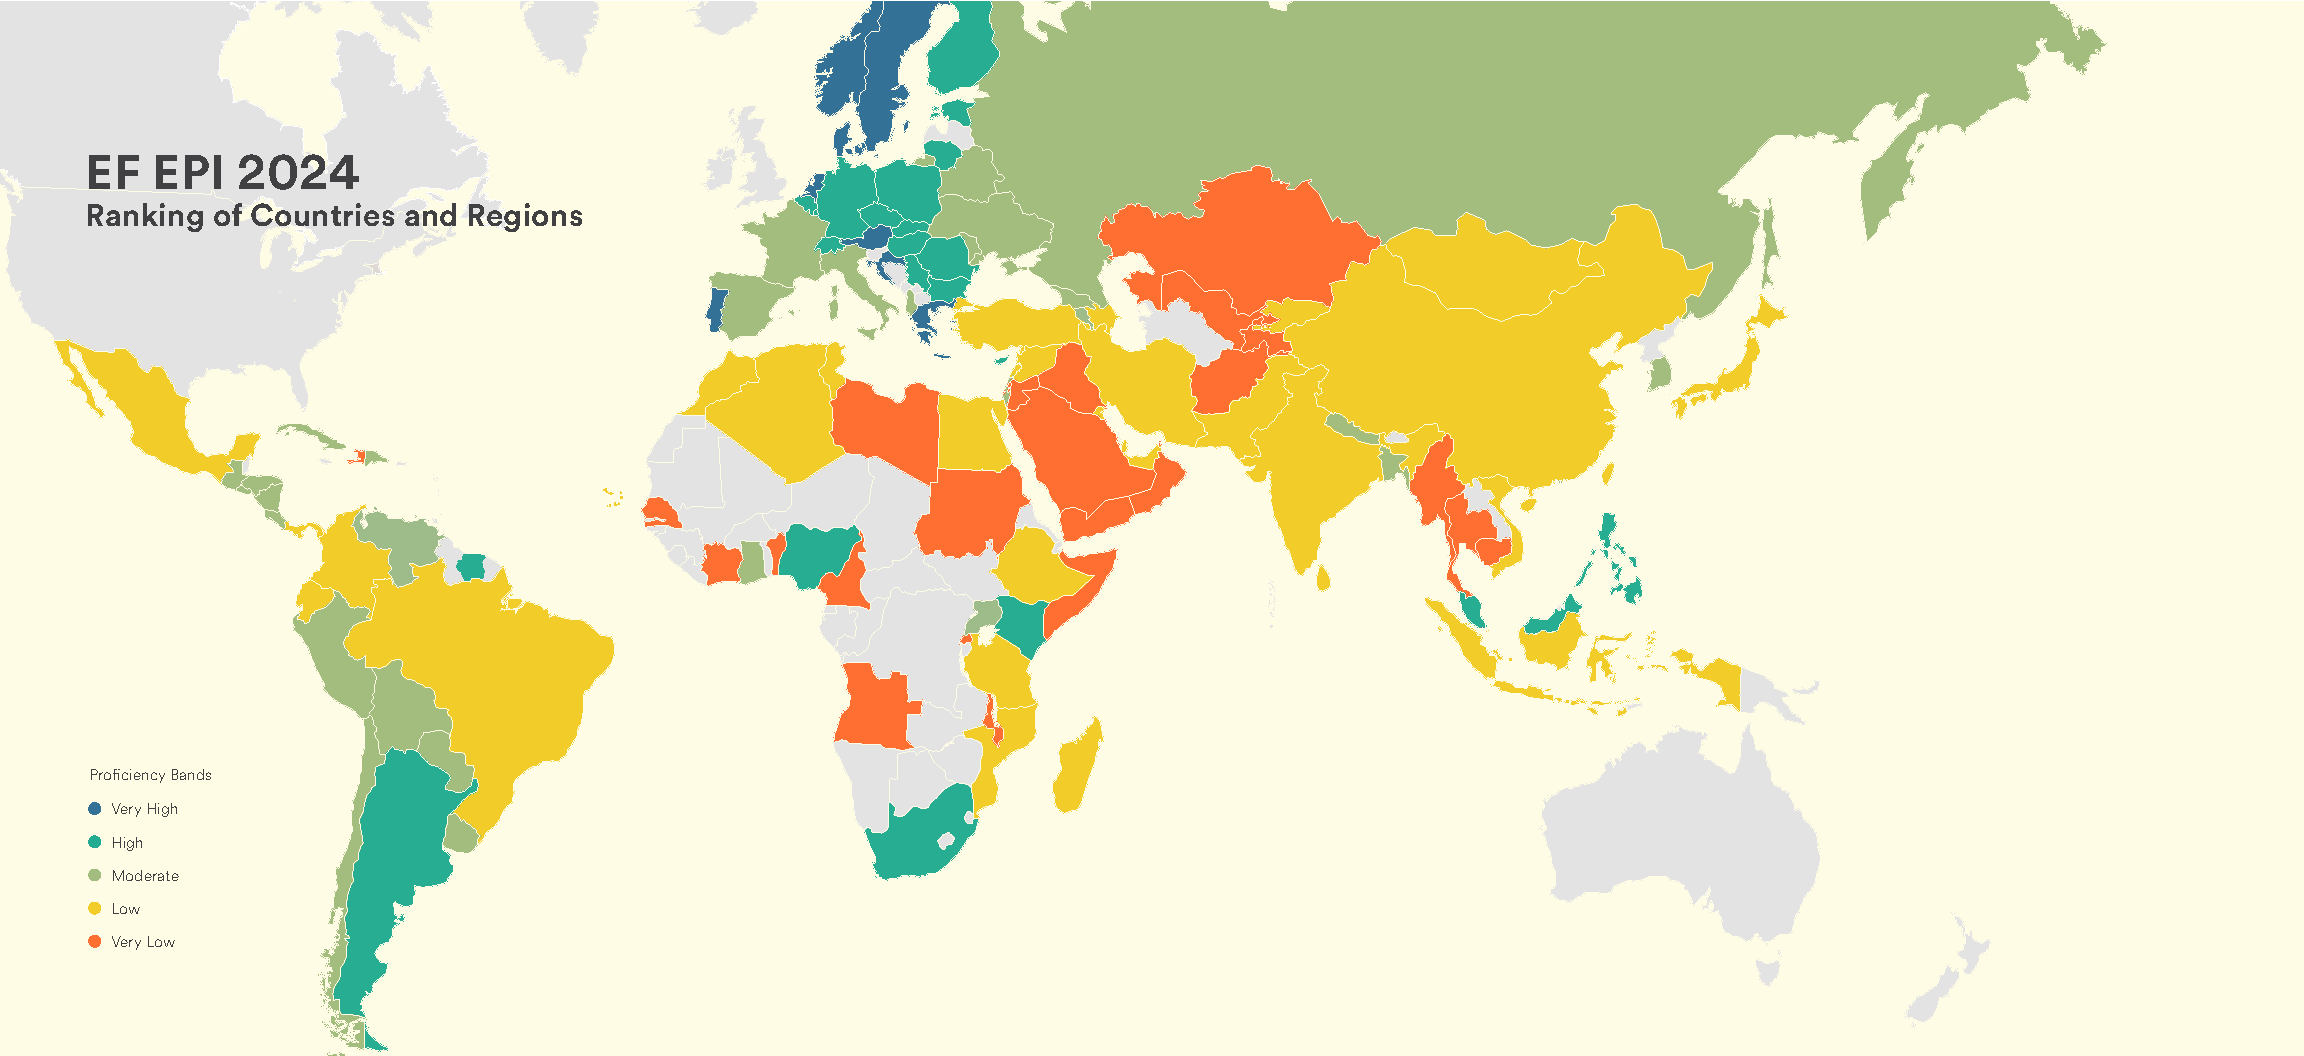
\includegraphics[width=\textwidth]{figures/ef-epi-2024-english-crop.pdf}
      \begin{textblock*}{8cm}(\paperwidth-9cm, \paperheight-2.5cm)  % (x,y) coordinates from top-left
        \textbf{\Large $> 1.4$ billion speakers}

        \textbf{\Large $\sim 75\%$ non-native}
      \end{textblock*}
    \end{center}
    \caption{English Proficiency bands by countries \citeyear{ef-epi-2024}}\label{fig:ef-epi}
  \end{figure}
\end{frame}

\note{
  English is one of the most widely used languages globally,
  spoken by approximately more than 1.4 billion speakers, with almost 75\% of them being non-native speakers
  As the number of esl and efl learners continues to grow, the need for effective language learning tools and resources has increased significantly.
  However, grammatical and spelling errors remain common challenges for many writers, affecting clarity and professionalism.
}

\subsection{Definition}

\begin{frame}{Definition of Grammatical Error Correction}
  \centering
  {\Huge
    \textcolor{red}{G}rammatical
    \textcolor{red}{E}rror
    \textcolor{red}{C}orrection
  }

  \vfill

  {\Large
    He \textcolor{red}{go} to the store and \textcolor{red}{buyed} some \textcolor{red}{apple's}.
  }

  \noindent\rule[0.5ex]{\linewidth}{1pt}

  {\Large
    He \textcolor{green}{goes} to the store and \textcolor{green}{bought} some \textcolor{green}{apples}.
  }

  \vfill
\end{frame}

\note[itemize]{
  \item Grammatical Error Correction, or GEC, is the task of automatically detecting and correcting errors in text.

  \item Despite its name, the task is not limited to grammatical errors, such as missing prepositions and mismatched
  subject-verb agreement but it also expect to fix orthographic and semantic errors, such as misspellings and word choice errors.

  \item The term Grammatical Error Correction is thus something of a misnomer but is nevertheless now commonly understood to encompass errors that are not always strictly grammatical in nature.

  \item A more descriptive term is Language Error Correction.
}

\subsection{Usage barriers}

\begin{frame}{Usage barriers}
  \begin{itemize}
    \item Command-line interface
    \item Requires capable hardware
  \end{itemize}

  \pause

  \vspace{1cm}

  {\Large $\Rightarrow$ Solution: A lightweight web interface}
\end{frame}

\note[itemize]{
  \item Despite significant recent advancements in GEC technology, many sota systems remain inaccessible to the general public due to their reliance on command line interfaces and high performance computing resources.

  \item This creates a barrier for non technical users, particularly those in developing countries with limited access to advanced technology and slow internet connections.

  \item This is where GecWeb comes in, it provides a lightweight, user friendly GEC system that can be easily
  accessed via mobile devices or low-end computers.
}
